\documentclass[12pt]{article}
\renewcommand{\labelitemii}{$\star$} 
\usepackage[margin=10pt,font=small,labelfont=bf,labelsep=period,hypcap=false]{caption}
\usepackage{graphicx}
\usepackage{natbib}
\renewcommand{\bibsection}{\section{\refname}} 
\usepackage{attrib}
\usepackage{lmodern}
\usepackage{supertabular}
\usepackage{pifont}
\usepackage{enumitem}
\DeclareGraphicsExtensions{.pdf,.png,.jpg}
\usepackage[bookmarks=true,colorlinks=true,linktoc=page,linkcolor=blue,citecolor=blue]{hyperref}
\parindent0pt \parskip8pt
\overfullrule=2cm
\begin{document}

\title{\vspace{-.5in}
USF Spike Sorter User Guide}
\author{Dr. Lauren Segers\and Dr. Sarah Nuding\and Russell O'Connor\and Dr. Chris Wilson}
\date{\today}
\maketitle

This document is an overview of the USF Spike Sorter's suite of tools
for processing, evaluating and reviewing clusters.  Please feel free
to add comments/critiques so that we can improve the tutorial and make
it easier for anyone interested in learning how to use this software.

\vspace{.5in}

\begin{quote}
{\itshape ``What about miracles?}

Finally, we want to give a very strong warning. A spike sorter is a
machine to separate spikes on the basis of their waveform. This could
in principle be done by a human being. One should bear in mind that,
when the spike signals are so noisy that many of one's careful sorting
decisions are turned into nonsense, the spike sorter will generate the
same nonsense, only at a considerably higher rate.''
\attrib{\cite{kreiter1989low}}

\begin{quote}
\end{quote}

When in doubt, throw it out.
\attrib{Lindsey, personal communication}

\begin{quote}
\end{quote}

Corollary: ``Doubt must be earned.''
\attrib{Nuding, added in proof}

\end{quote}
\tableofcontents

\clearpage
\section{Introduction}

Over the last few decades, multiple-unit extracellular recordings from
the CNS have become important for understanding the patterns of
information flow between and within neuronal assemblies. Initially,
single-cell recordings (either intra- or extra-cellular) were used to
characterize the behavior of a neuron. As extracellular electrode
technology advanced and the ability to record multiple isolated units
(on one or many electrodes) has become commonplace, however, the
development of analysis tools to facilitate the identification and
classification of multiple units has lagged when compared to the
ability to record multiple cells.

The chief problem one faces when recording from multiple extracellular
units over time is the waxing and waning of signal strength due to
multiple factors that change the spatial relationship between
electrode and neuron. Early analysis of single units consisted of an
analog amplitude/threshold window discriminator (Schmitt trigger). \
The next evolution included a time window to allow discrimination of
more than one neuron with similar action potential amplitudes (e.g.,
Bak spike sorting modules). With the evolution of digital computer
technology, sophisticated cluster cutting software has become
increasingly feasible (e.g., \cite{fee1996automatic},
\cite{lewicki1998review}, \cite{gerstein1964simultaneous}).

The \textbf{USF Spike Sorter} package represents a semi-automatic
iterative approach for sorting distinct sets of wave forms, evaluated
in a 64 dimensional space, with each resulting set of clusters
representing the separable ``spikes'' from one or more single neurons
recorded with a particular electrode.

The Spike Sorter currently provides facilities for the parallel
automatic sorting of signals from up to 128 electrodes in one or more
multi-electrode arrays and the subsequent merger of the separate time
series into a single file together with other analog signals for later
analysis.

This guide is intended to help the user become familiar with the steps
of data analysis used by the Spike Sorter package. This procedure
involves several steps:
\begin{itemize}
\item First, the large data file is \textbf{Split} into its component
  128 channels; these are called ``chan files.''
\item Common 60 Hz noise sometimes found in these types of recordings
  must be removed, in a step called \textbf{Cleaning}.
\item The next step is \textbf{Autosort processing,} where the Spike
  Sorter performs user-designated work on each channel to separate the
  spikes on each unit channel into clusters, or integrate or digitize
  analog data (and, if desired, produce pulses indicating the
  beginning of inspiration and expiration using the phrenic nerve
  channel, cardiac pulses, and/or tracheal pulses).
\item Next, the clusters are assessed by users. Each cluster is
  accepted as is, merged with other clusters, or deleted. This is
  called the \textbf{Evaluating - Manual sorting} step.
\item {\bfseries Editing\textmd{ must be performed on most clusters to
      yield the most accurate representation of that cell's activity.
      This involves use of the auxiliary programs discussed in Section
      \ref{aux}.}}
\item \textbf{Reviewing} is then performed on the edited clusters, as
  varying opinions made regarding subjective judgments are
  unavoidable.
\item All the data are then \textbf{Merged} into one file and
  subjected to quality control procedures (\textbf{QC'd}).
\end{itemize}

\textbf{THE TUTORIAL:} We have a collection of ``tricky''
channels---clusters with errant waveforms within them that must be
removed, waveforms that gradually change during the recording,
single-unit spikes segregated into different clusters because of their
relative position in bursts, I and E cells with similar waveforms that
make clean clusters when merged but they SHOULD not be
merged{}---typical gotchas you must be aware of while sorting. It is
crucial that new users complete this tutorial to see how all the
pieces of the Spike Sorter work together -- \textit{to create the most
  accurate representation of the cell's activity.}

\section {Split the files}

Each recording consists of one or two files. Each file contains 64
channels of data. The first processing step splits the data into
individual files -- one file per channel. These files are called
``chan files.''

\begin{itemize}
\item For USF experiments, create a directory named with the
  experiment date (e.g., 2004-01-18) within {\tt /raid/datamax} on
  cisc3.  This directory will be referred to as the \textbf{data
    directory} for this experiment. Copy the {\tt .daq} files from the
  recorder, tape, or other source to the data directory by your
  preferred method. (This step may already be done. There is no need
  to make a second copy of the files.)
\item Open a command line window and go to the directory into which
  you just put the {\tt .daq} files. For example,
  \begin{verbatim}
cd /datamax/2004-01-18
  \end{verbatim}
\item Run the {\tt split\_all.sh} script to split the {\tt .daq} files
  into separate channels by typing
  \begin{verbatim}
split_all.sh 001 002 003
  \end{verbatim}
\item This runs the {\tt daq2\_split} program for all the
  recordings. The script will look for both 1-64 and 65-128 files, but
  it is not an error if any of these do not exist. The {\tt
    daq2\_split} program will create split directories and then split
  the data into separate chan files.
\end{itemize}

NOTES:
\begin{itemize}
\item Splitting is I/O intensive. It's best if splitting occurs on the
  machine where the data are (i.e., cisc3).
\item Split the file you need when you need it.
\end{itemize}

{\bfseries Consult the {\ttfamily Daq2CleanUsersManual.pdf} for specific
  instructions on how to split the files.}

\section {The ``Cleaning'' pre-processing option}

Recordings may have common noise. This package optionally employs
digital filtering and removal of nonspike-like noise common to the
electrodes in an array before applying the 64-space algorithm. This
pre-processing uses a slightly modified version of a (MATLAB/Octave)
``cleaning'' application developed in the laboratory of George
Gerstein \citep{musial2002signal} applied to blocks of channel
recordings with spike data or nerve (multi-unit) recordings to remove
any noise that doesn't look like a spike that the blocks have in
common. Typically, blocks of 8 or 16 {\tt *.chan} files are
cleaned. Note: at least 3 ``nerve'' channels (i.e., concurrent
recordings from afferent and/or efferent peripheral nerves) must be
recorded to have a useful block of nerve channels for cleaning
purposes. See the separate documentation for details on the cleaning
procedure.\textbf{ Note: channels with blood pressure, tracheal
  pressure, end-tidal CO$_2$}\textbf{, or other ``non-neural''
  measurements are typically NOT cleaned as this process may distort
  the signal.}

NOTES:
\begin{itemize}
\item Sometimes/often it is easier to \textbf{copy} chanlists from
  time-adjacent experiments/recordings rather than start from scratch
  (look for a chanlist on {\tt /datamax})
\item Be sure chanlists are appropriate for your recording.
\item \textbf{Cleaning is CPU intensive} and is performed by one
  machine. Up to 8 processors will be used for cleaning. Think about
  using cisc1, cisc4, or cisc5 for cleaning -- they have lots of
  processors.
\end{itemize}
{\bfseries Consult the {\ttfamily Daq2CleanUsersManual.pdf} for
  specific instructions on how to clean the files.}

\section {Autosort processing}

Autosort processing includes the following steps:
\begin{itemize}
\item Automatic determination of a detection threshold that makes
  non-spike regions maximally Gaussian
\item Identification of waveform peaks that are likely to belong to
  spikes
\item Automatic determination of the number of discriminable spike
  waveforms (to be used as templates) using a mean shift clustering
  algorithm \citep{georgescu2003mean} on a whitened unreduced feature
  space of 64-sample waveforms with sub-sample alignment of waveforms
  by sinc interpolation.
\item Spike detection and classification by least-squares template
  matching to potential spike waveforms
\item Separation of loosely overlapped spikes by peak matching and
  template subtraction
\end{itemize}


In this version of the Spike Sorter, the user's task is to manually
merge or delete the clusters resulting from Autosorting. Note that one
or more clusters may require additional editing before they can be
joined.

\subsection {Channel Work Assignments, Labels, and Numbers text files
  and the Prefix}

The {\tt spikesort\_control\_panel} program is started from the
command line with one argument: \textbf{the absolute path to the
  location of the cleaned chan files and the prefix. }


On the Spike Sorter control panel, each channel has two one-letter
fields that specify the work to be done on the channel, followed by
one label field, followed by a number field that specifies the range
to be used for cell ID's for any cells found on that channel (see
\textbf{Fig. \ref{initial}} below). The information for each of those
fields is found, respectively, in the \textbf{\ttfamily{*.wrk}},
\textbf{\ttfamily{*.lbl},} and \textbf{\ttfamily{*.num}} text
files. In each of these filenames, the \textbf{\ttfamily{*}} stands
for the \textbf{filename prefix} for that particular
experiment. \textbf{The prefix is a string that all relevant filenames
  start with for that experiment.} For example, for USF data, the
prefix is composed of the experiment date (eg., 2004-01-18) and the
recording number (say it's the first recording of the experiment)
joined with an underscore, like this: 2004-01-18\_001. (This string
may also occasionally be referred to as the experiment name.) For
example, if your experiment prefix is 2004-01-18\_001, the data
directory location is likely to be {\tt
  /datamax/2004-01-18/clean.001/}, and the 3 text files will be named
{\tt 2004-01-18\_001.lbl}, {\tt 2004-01-18\_001.num}, and {\tt
  2004-01-18\_001.wrk}.

Spike Sorter expects the {\tt .wrk}, {\tt .lbl}, and {\tt .num} files
to be present in the folder with the clean chan files (but can get by
with just the label file if necessary. In that case, default values
for the work and number fields are set based on the label if the label
is recognized by the control panel; if the label is not recognized,
the work and number fields will be blank).

The format for each of these text files is simply one line per
channel. For a recording with 4 channels, recorded using the Pegasus
electrode array in the pons and the Medusa array in the raphe along
with phrenic nerve activity, the text files could look like this:
\begin{center}
\begin{tabular}{|c|c|c|}
\hline
{ the {\tt .wrk} file} & { the {\tt .lbl} file} & { the {\tt .num} file}\\
\hline
\hline
{ S-} & { Pegasus 1} & { 501-599}\\
\hline
{ S-} & { Pegasus 2} & { 501-599}\\
\hline
{ S-} & { Medusa 1} & { 901-996}\\
\hline
{ IR} & { N1} & { 1}\\
\hline
\end{tabular}
\end{center}

{\bfseries Make sure that the information in these text files matches
  the data for THIS experiment and THIS recording (i.e., check the day
  sheets!).}

The {\tt .wrk}, {\tt .lbl}, and {\tt .num} files can be created or
changed in several ways. They can be
\begin{itemize}
\item copied from a previous experiment and renamed (this saves having
  to type it all in again), or
\item created/edited using a text editor, or
\item created/edited within the Spike Sorter control panel
\end{itemize}

One more time: Be sure the files are named correctly and reside in the
directory with the clean chan files.

Note: Don't edit the files using a Windows program unless you know how
to preserve the format, including not adding CR characters to the line
endings. Using an editor like {\tt gedit} or {\tt emacs} is a good
choice.

If you use the control panel to make changes to a channel's work
assignment(s), label, or ID number range, \textbf{you must hit the
  Enter key after each change to register the change within the
  control panel display and cause the corresponding text file to be
  re-written.} However, if you are adding new channels above the
existing channels, editing within the control panel won't work well
and you are better off using a text editor to add the new channel
information to the {\tt .wrk}, {\tt .lbl}, and {\tt .num} files.

\subsection {The {\tt host\_list} file}

The {\tt host\_list} file (located in {\tt /etc/spikesorter}) is a
list of computers (and the CPUs on each computer) that Spike Sorter is
allowed to use to do the work of Autosort processing. It's a good idea
to open this file with {\tt gedit} to be sure that all available
processors are listed. If necessary, you can remove processors and
computers that are not currently available.

You may create or edit this file using {\tt gedit}. It might look like
this:
\begin{verbatim}
cisc2_0 fs /datamax
cisc2_1 fs /datamax
cisc2_2 fs /datamax
cisc3_5 fs /datamax
cisc3_6 fs /datamax
cisc3_7 fs /datamax
\end{verbatim}

The above information is telling Spike Sorter to use the first 3 CPUs
on the computer named {\tt cisc2} (note the zero-based numbering) and
the sixth, seventh, and eighth CPUs on {\tt cisc3}. Include {\tt fs}
on each line to indicate which method Spike Sorter will use to access
each work computer (it's always {\tt fs}); {\tt /datamax} is a pointer
for each work computer to the data directory (it's {\tt /datamax} or
{\tt /zbox} for USF data).

The computers listed in the {\tt host\_list} file are doing the work
of Autosorting and {\bfseries the working directories are located on
  these computers in {\ttfamily /home/ssu}.  } Along with other files,
you will find the {\tt .edt} file for each channel in the working
directory when Autosorting is complete and during the Manual sorting
process. An {\tt .edt} file is a list of cluster ID numbers and
occurrence times in 0.1 msec bins.

\subsection{Starting the Spike Sorter Control Panel}

The Spike Sorter is run from a Linux-based computer, currently one of
the {\tt cisc} computers. \textbf{Log in as \ttfamily ssu} (spike
sorter user) before running Spike Sorter. You can ``become'' ssu by
logging in via the login screen or by entering text of the following
form on the command line in a new terminal window (NOTE: do not
navigate to the experiment directory):
\begin{verbatim}
ssh -Y -l ssu name_of_computer
\end{verbatim}
Examples:

to run Spike Sorter on cisc5:
\begin{verbatim}
ssh -Y -l ssu cisc5
\end{verbatim}
to run Spike Sorter on the machine you're already logged onto:
\begin{verbatim}
ssh -Y -l ssu localhost
\end{verbatim}

The password for ssu is \textbf{\ttfamily Obex@3040.}

The command to invoke Spike Sorter control panel is of the form
\begin{verbatim}
spikesort_control_panel path_to_clean_chan_files/prefix
\end{verbatim}

For USF data, the command is more specifically of the form

\makebox[\textwidth][c]{{\tt spikesort\_control\_panel
    /datamax/experimentdate/clean/experimentdate\_recordingnumber}}

Here is a really specific example for the first recording of
the experiment named {\tt 2004-01-18}:

\makebox[\textwidth][c]{{\tt spikesort\_control\_panel
    /datamax/2004-01-18/clean.001/2004-01-08\_001}}

For USF data, note that the date must be in {\tt yyyy-mm-dd} format
and recording numbers must have three digits. Be aware that if more
than one recording exists for an experiment date, you may find more
than one directory of cleaned {\tt .chan} files; in that case, the
directories will be named {\tt clean.001}, {\tt clean.002},
etc. {\bfseries The important thing to remember here is that you must
  tell the Spike Sorter where to find your clean {\ttfamily .chan}
  files and you must supply the prefix.}

(\textbf{Note}: The path in this command must point to the location of
your cleaned {\tt .chan} files (i.e., the data directory), so if you are
running the Spike Sorter on a non-USF computer network, you may have
to supply a different path. {\bfseries You must tell the Spike Sorter
  control panel where to find your clean {\ttfamily .chan} files and
  tell it the correct prefix for that experiment.})

A small window will appear briefly as the dispatching computer
communicates with each of the assigned work computers and
processors. If communication fails, you'll see a {\sf timed out}
message for that processor, and Spike Sorter will proceed to the next
processor in the list.

Spike Sorter control panel will be seen (\textbf{Fig. \ref{initial}}).


\bigskip

\begin{center}
\makebox[\textwidth][c]{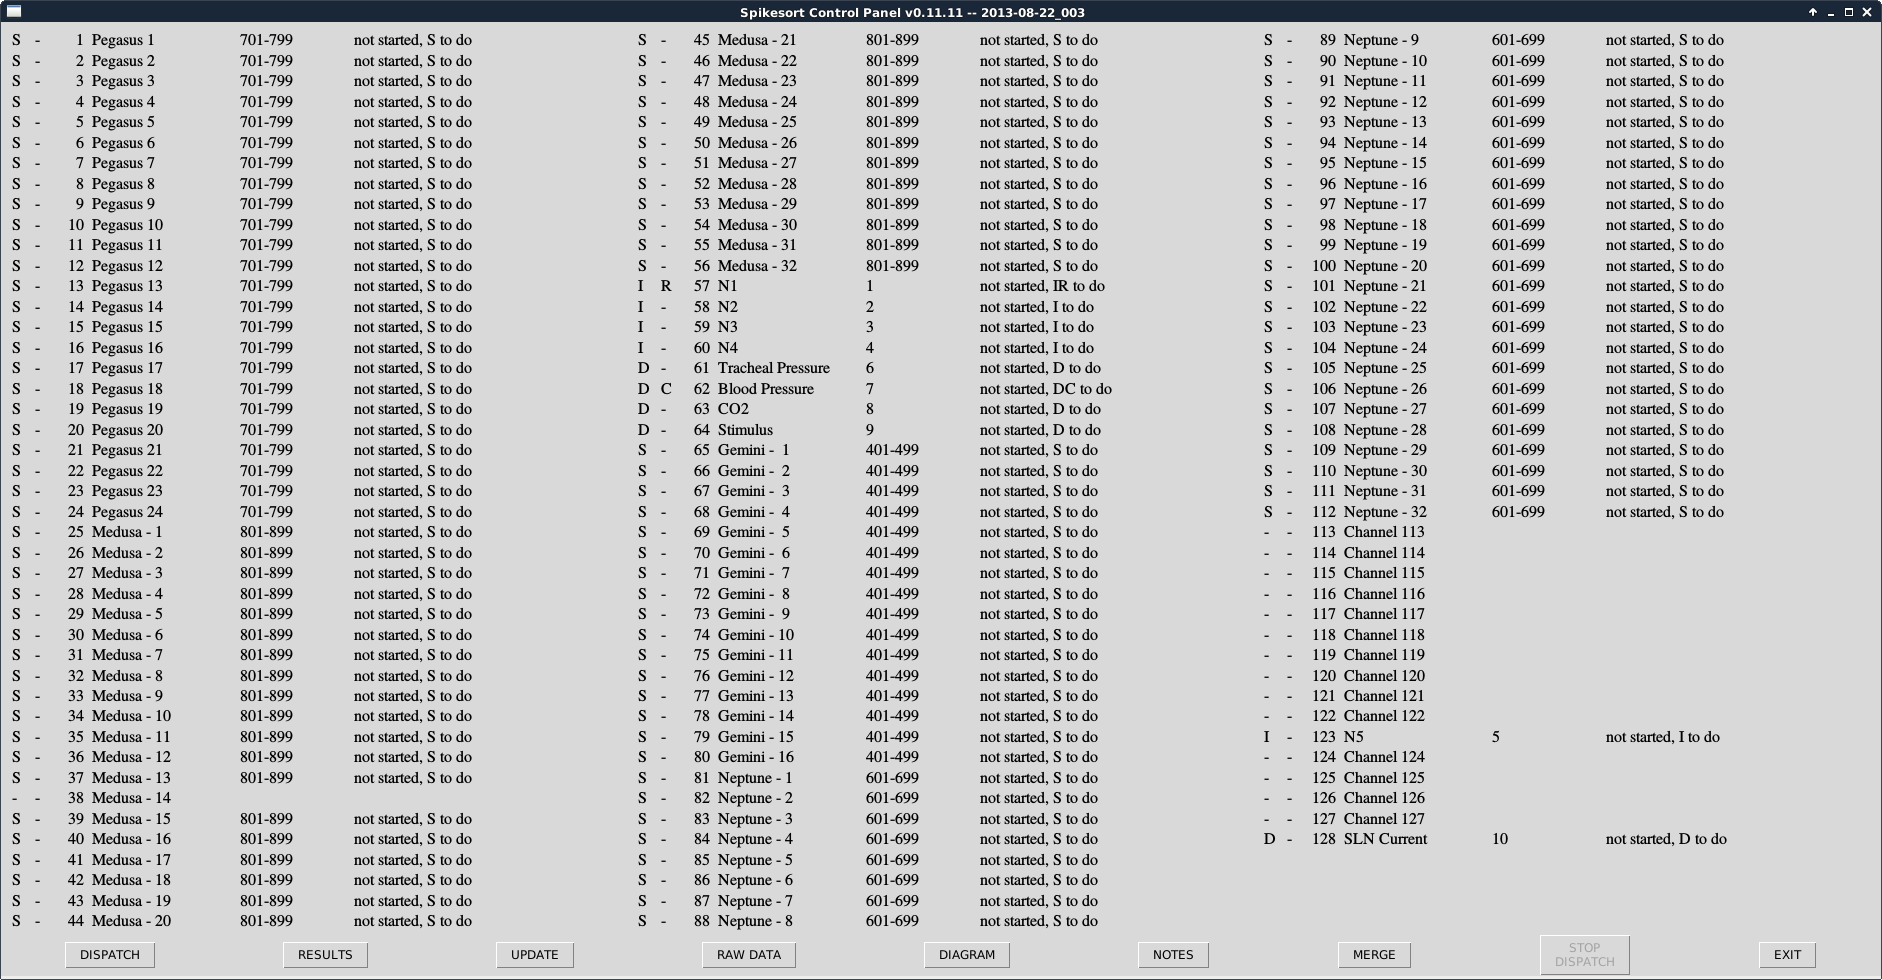
\includegraphics[width=6.9591in]{userguide-img001.png}}
\captionof{figure}{The control panel before Autosorting has
  been dispatched. The control panel for the Spike Sorter allows the
  user to designate work assignments, view ``raw'' data, obtain
  ``reference frame'' diagrams, and launch the Autosort work
  assignments. Note that no work assignment was made for channel 38 in
  this example; the day sheets for this recording state that the motor
  for this electrode was not working.}
\label{initial}
\end{center}

In the control panel, you will see a list of all the channels in this
format:

{\centering
- -\hfill Ch\#\hfill ARRAY-\#\hfill MERGED CHANNEL RANGE\hfill STATUS
\par}

The 5 columns in the control panel contain:

\begin{itemize}
\item Default work assignments. Assign the work to be performed on
  each channel (based on what kind of data is on that channel, like
  extracellular activity, nerve recording, analog data like blood
  pressure, etc.). This information is in the {\tt *.wrk} file.
\begin{description}
\item[S -] = spike sort, used on electrode array channels
\item[I -] = {integrate} (high speed digitizing, looks like a raw
  signal); used on nerve hannels
\item[I R] = integrate and create respiratory (I and E) pulses; used
  on the phrenic nerve channel (note: do I and R on only one phrenic
  channel -- if more than one phrenic channel is available, choose the
  better one)
\item[D -] = digitize (low speed digitizing); used on an analog
  channel that is not a nerve channel (e.g., the CO$_2$ and stimulus
  channels)
\item[D C] = digitize and make cardiac pulses; used on the blood
  pressure channel
\item[D T] = digitize and make tracheal pressure pulses; used on the
  tracheal pressure channel
\end{description}
\item Channel number (1 to 128).
\item Array name and electrode number. For example ``Pegasus 6.'' This
  information is contained within the {\tt *.lbl} file.
\item Merged channel range. The default is 001 -- 996. The correct
  range must be assigned according to brain region; this information
  is on the hard copy of the protocol detail (``day sheets'') made at
  the time of the experiment. To assign, select the channel(s) to be
  assigned (you may use the Shift and Ctrl keys to select a range or
  individual channels), right-click on the merged channel range for
  any of the selected channels, hold the right button down to choose
  the appropriate brain region, \textbf{then hit ``Enter'' on the
    \textit{keyboard} (not the number pad)}. The channel ranges may be
  assigned at any time before creating the {\tt .edt} file for the
  entire multi-channel recording. (Note: The merged channel range can
  also be assigned by editing the {\tt *.num} file.)
\item Channel status. Options are ``not started, \_ to do'',
  ``running'', or ``done'' using the assigned work. If this text is in
  red, there's usually an issue that you must address.
\end{itemize}

\paragraph{Work assignments:} The letter in the first column
indicates the work that the Spike Sorter will perform on that channel.
Once the control panel is running, you can select a channel by
clicking on the left-most letter. It will already have an ``S'',
``I'', or ``D'' (or a ``-''). Left click with the mouse to cycle
through the letters:

{\centering
\begin{tabular}{ll}
\textbf{S }= spike sort & \textbf{D }= digitize \\
\textbf{I }= integrate &  \textbf{-} = do nothing\\
\end{tabular}\par}
After verifying that the work assignment for each channel is correct,
click the {\sf DISPATCH} button to begin Spike Sorter Autosort
Processing. You will see the channel status change, for example, from
``not started, S to do'' to ``running on cisc3\_2: \#\#\#\#\#\#''. In
this example, the processing for this channel was assigned to the
second processor on cisc3; the number displayed at the end of the
phrase will grow larger as processing proceeds. Once a channel has
been dispatched to a working computer, the status is updated to
include that information. So now you know where to find the working
directory for each channel. In this example, the working directory is
on cisc3 in {\tt /home/ssu}.

Processing can take up to a few days for a long recording with many
different waveforms. \textbf{Check the control panel regularly to see
  if there are any problems.} Red text in the status line should be
investigated.

You may stop Autosorting by clicking the {\sf STOP DISPATCH} button.
This will not stop channels that are already running, but it will
prevent any ``not started'' channels from being started.

{\em If the Spike Sorter is running slowly or ``taking forever'' on a
  particular channel, then look at the ``raw'' signal (see Section
  \ref{wave} for how to use the {\tt waveform.tcl} program). If visual
  inspection suggests that there is no clear cell activity, you can
  stop processing on that channel by going to the machine it is
  running on and killing the appropriate {\tt spikesort} process. This
  would be a good time to delete all the files associated with that
  channel.  Then click {\sf STOP DISPATCH}, change the work assignment
  for that channel to ``-- --'', and click {\sf DISPATCH}).}

If channels are waiting to be Autosorted, do not close the control
panel; let it complete the work assignment for each channel. It's
important for the dispatching computer to finish the job. If you
re-start the control panel for the same experiment on another machine
with a different {\tt host\_list} and dispatch again, the results will
be very confusing.  If the dispatching control panel crashes (or is
closed by mistake), Autosorting will continue on the channels that
were dispatched before the control panel stopped. The next time you
open the control panel on the dispatching computer, the status for
each channel will be reported; if some channels are reported to be
``not started,'' clicking the {\sf DISPATCH} button will begin the
Autosorting process on those channels.

\textbf{Do not use the dispatching control panel to Evaluate channels
  until all channels have been Autosorted.} However, you may open
\textit{another} control panel before every channel has been
Autosorted to Evaluate channels for which Autosorting is finished.

\textbf{NOTE}: An {\tt .edt} file is written to the working directory
for each channel by the Autosort Process. An edt file is a list of
cluster ID numbers and occurrence times in 0.1 msec bins. We have
several auxiliary programs that use an {\tt .edt} file as input. For
example, looking at an {\tt .edt} file with {\tt autoCCH} (which will
show you the cross-correlation function for 2 clusters) will help you
with the Evaluating/Manual Sorting process. Analysis of intermediate
{\tt .edt} files optionally created as you merge and delete clusters
will be very useful as well; however, be aware that previous edt files
written for this channel will be overwritten with no warning unless
you have renamed them.

\clearpage
\section{Evaluating - Manual Sorting}

Once the \textbf{Autosort Processing} has been completed,
\textbf{Evaluating} can begin. Note that a processed channel can be
evaluated even if other channels are still being processed. In order
to do so, a second control panel must be used (this is easier if you
use a different ``Desktop'' to open each subsequent control panel).
An example of a control panel while Autosort is running is shown in
\textbf{Fig. \ref{running}}.


\begin{center}
  \makebox[\textwidth][c]{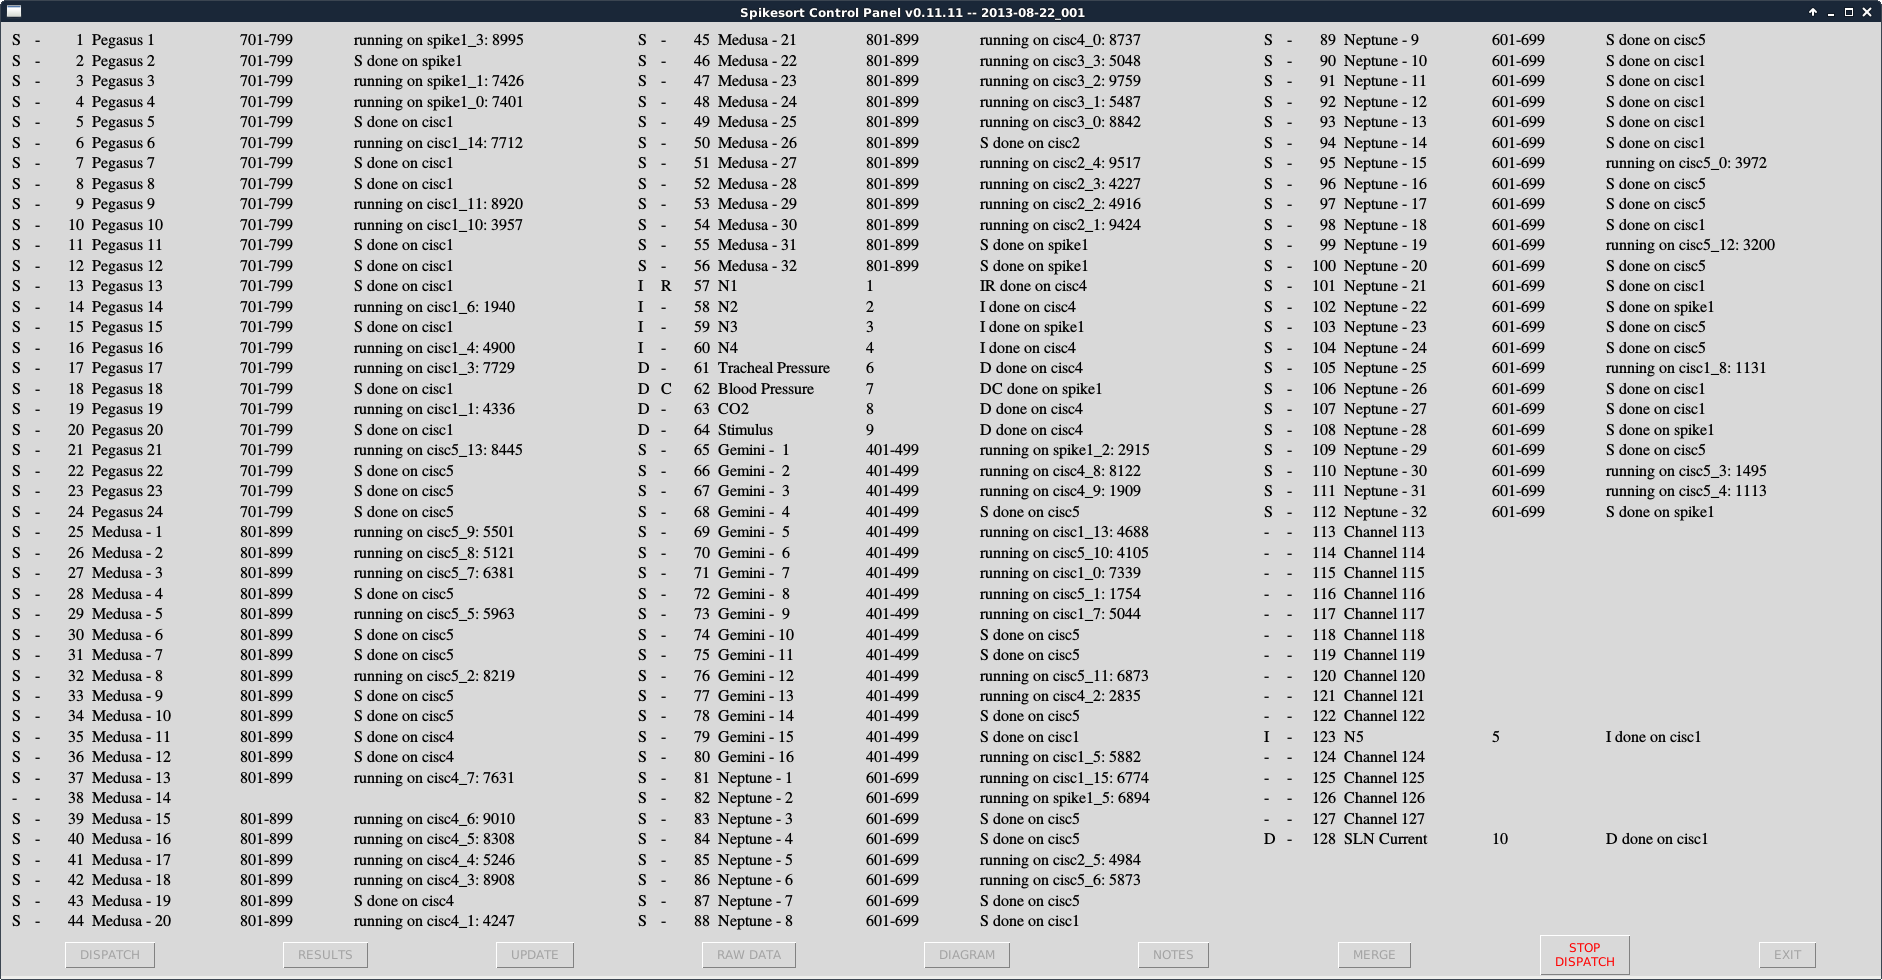
\includegraphics[width=7.1307in]{userguide-img002.png}}
  \captionof{figure}{The control panel while Autosort is running.}
  \label{running}
\end{center}
If a channel is red, either there is a problem with the channel or it
has been selected by the user. If, for example, ``S done on cisc5'' is
seen, this means that the Spike Sorter has finished autosorting this
channel using a processor on computer cisc5; the working directory for
this channel is on cisc5 in {\tt /home/ssu}. ``SE done'' indicates
that an {\tt *.edt} file has been written once for this channel; ``SEE
done'' means that an {\tt *.edt} has been written twice.

At the bottom of the control panel, the buttons relevant to Evaluating
are as follows:

\begin{description}
\item \textbf{\textsf{DISPATCH}} -- Once the channels have been
  assigned, the {\sf DISPATCH} button begins the Autosort processing
  of the data.
\item \textbf{\textsf{RESULTS}} -- Opens the USF Spike Sorter
  window.\textsf{\textcolor{black}{ }}The \textsf{RESULTS} button will
  take you to the \textsf{Spikesorter} panel showing cut clusters and
  autocorrelation histograms, and will allow access to most of the
  tools you'll need to evaluate clusters for merging or deleting.
\item \textbf{\textsf{UPDATE}} -- Used to update the status column in
  the control panel. Use this once an {\tt *.edt} has been made to
  change ``S'' to ``SE.''
\item \textbf{\textsf{RAW DATA}} -- Displays the raw data for a
  selected channel (\textbf{Fig. \ref{raw}}). If you have selected a
  time period in the \textit{Timeline} (see Section \ref{timeline}),
  then the raw data display will initially show that segment of
  data. If you have nothing selected in the \textit{Timeline}, then
  the whole data file is displayed.
\item \textbf{\textsf{DIAGRAM}}-- The Spike Sorter software makes an
  effort to align the clusters in relationship to each other and
  displays this information as a series of circles labeled with the
  cluster number that they represent linked by arrows.  The number
  over each arrow is the estimated ``distance'' between the centers of
  the 2 clusters (expressed as the number of standard deviations of
  the noise).
\item \textbf{\textsf{NOTES}} -- Allows users to communicate about the
  channel or decisions made during the manual sorting; comments are
  stored in an electronic file.
\item \textbf{\textsf{MERGE}} -- Creates a large file containing all
  of the information from each channel. Please make sure that all
  processing has been completed, all merged channel numbers have been
  assigned, and that individual {\tt *.edt} files have been written
  for each channel.  Also, be sure that the array coordinate
  spreadsheet is completed, QC'd, and in the appropriate folder before
  pressing this button (for USF, the appropriate folder is {\tt
    /raid/experiments/experiment\_name}). \textbf{Note: Clicking the
    {\sf MERGE} button is typically the last thing you do in the Spike
    Sorter.}
\item \textbf{\textsf{STOP DISPATCH}} -- Halts any Autosort work that
  is being done (S, I, or D) on the channels.
\item \textbf{\textsf{EXIT}} -- Closes the control panel
\end{description}
\subsection{\sf RAW DATA}
The raw data display can be very helpful (visually as well as aurally)
in evaluating a channel. Selecting a channel in the control panel and
clicking on {\sf RAW DATA} will open a display similar to one seen
below (\textbf{Fig. \ref{raw}}). To listen to the trace -- as in a
live experiment with an audio monitor -- press ``p''. To stop the
audio, press ``s''.  The numbers in the upper-left and -right corners
are the time of the recording in seconds at the beginning and end of
the data displayed. The number in the upper-middle is the numbers of
seconds being displayed. Use the up and down arrow keys to zoom in and
out, and the left and right arrows to scroll through the raw data.
\begin{center}
  \makebox[\textwidth][c]{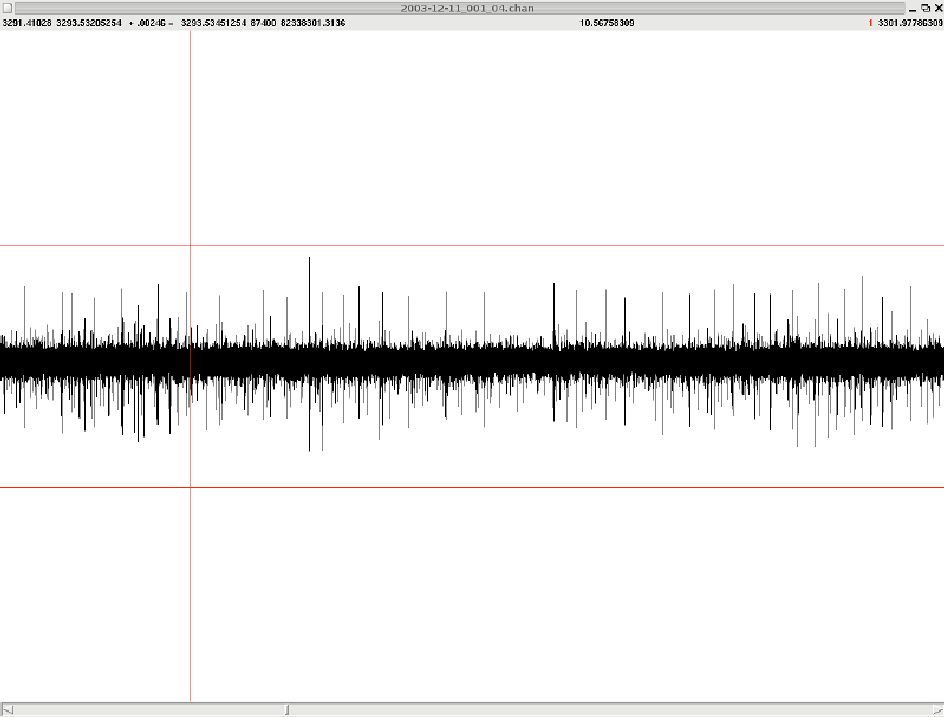
\includegraphics[width=7.1307in]{raw.png}}
  \captionof{figure}{Raw data viewer called from the \textsf{RAW DATA}
    button.}
  \label{raw}
\end{center}

\subsection{\sf DIAGRAM}
The Diagram \textbf{(Fig. \ref{diagram}}) is another tool that is
useful early in Evaluating. It can serve as a rough, preliminary guide
to aid merging of clusters by the user. Taking only the shapes of the
waveforms (and their ``alignment'' within the 64-sample window) into
consideration, the Spike Sorter makes an effort to display the
relationships between the clusters. Clusters that are not represented
in the diagram also require special consideration and may be other
units or unsortable signals. Clusters are displayed as numbers in
circles; units of SD of noise between them are displayed as numbers
above the arrows. Note: March, 2014 -- Russ anticipates changes in the
Diagram function; future versions of Spike Sorter will improve
waveform alignment.
\begin{center}
  \makebox[\textwidth][c]{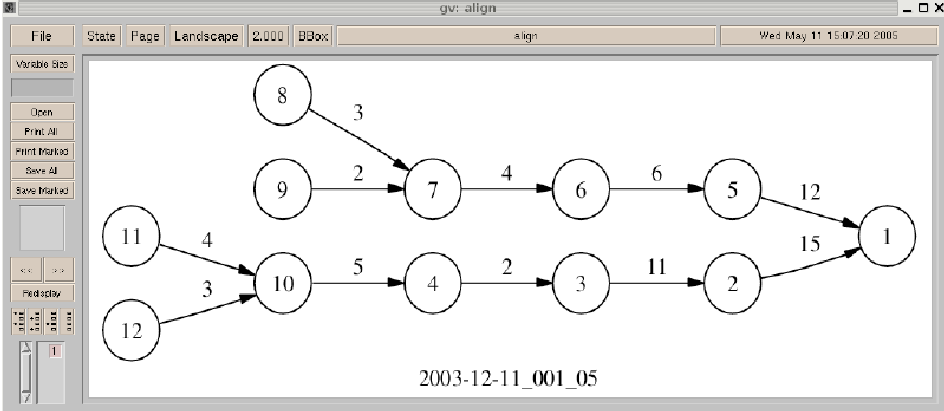
\includegraphics[width=7.1307in]{diagram.png}}
  \captionof{figure}{ The ``Diagram''. Note: This tool requires proper
    alignment of waveform clusters; future versions of Spike Sorter
    will improve waveform alignment.}
  \label{diagram}
\end{center}
\clearpage
\subsection{\sf RESULTS}
\subsubsection{Overview}
\label{overview}
To begin evaluating a channel, select that \textbf{channel number} on
the control panel, then click on \textsf{RESULTS}. The USF Spike
Sorter window will open (e.g., \textbf{Fig. \ref{results}}).
\begin{center}
  \makebox[\textwidth][c]{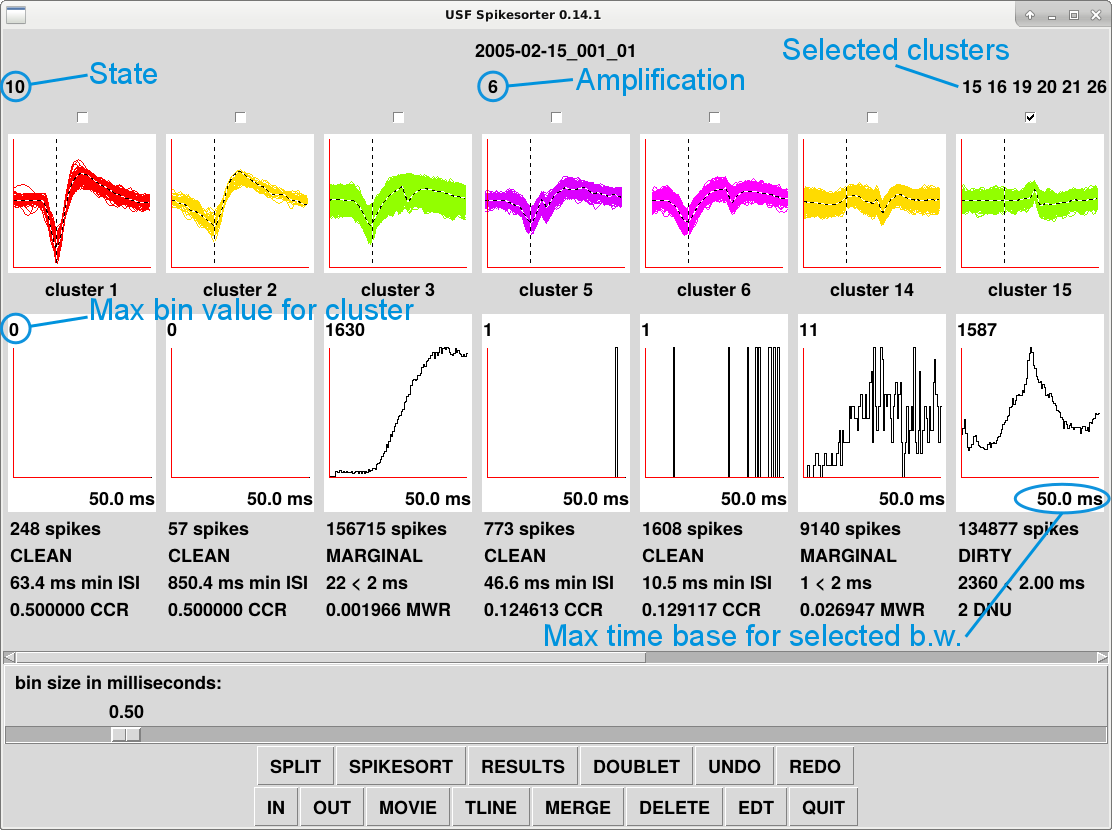
\includegraphics[width=7.1307in]{results.png}}
  \captionof{figure}{Screenshot of Spike Sorter Results Panel.}
  \label{results}
\end{center}
\clearpage

The results panel shows (from top to bottom and left to right):

\begin{itemize}
\item the \textbf{filename}
\item a ``\textbf{State}{}'' or configuration number (The Spike Sorter
  creates a new ``state'' any time a change is made to the data, such
  as a deletion or a merge, much like saving different versions of a
  file. This number is displayed in the upper left-hand corner. You
  can move back and forth in state space using the {\sf UNDO} and {\sf
    REDO} buttons -- see below)
\item the \textbf{amplification factor }(To increase or decrease the
  amplitude in the waveforms, use the ``+'' or ``-'' keys on the
  \textit{keyboard. }You don't have to use the Shift key; note that
  the keys in the keypad will not work.)
\item the \textbf{cluster number(s)} currently selected
\item a small \textbf{box} over each cluster (clicking within this box
  will select the cluster)
\item the cluster \textbf{waveforms} (The 64-sample waveforms
  displayed on this screen have had detected overlapping waveforms of
  other spikes subtracted from them. They are NOT the original (raw)
  traces displayed in the movie. Small waveforms not detected or
  subtracted may appear as ``warts'' or small bumps on the
  waveforms. The average of each cluster is superimposed over the
  waveform as a dashed line. The alignment point is shown as a
  vertical dashed line. See Section \ref{alignment} for alignment
  details.)
\item first-order \textbf{autocorrelation histograms} (also
  known as inter-spike interval histograms)
\item some \textbf{cluster information} including:
\begin{itemize}
\item number of spikes in the cluster
\item a ``clean/marginal/dirty{}'' assessment
\item the minimum inter-spike interval (ISI) or number of ISIs less
  than 2 ms
\item an inter-spike interval evaluation (CCR/MWR/DNU/EPR -- 
  \textbf{see Section \ref{cmd}}),
\end{itemize}
\item a \textbf{slider} to move left and right through the displayed
  clusters
\item a \textbf{bin size slider} to vary the size of the bins in
  milliseconds
\item the \textbf{function buttons:}
\begin{itemize}
\item \textbf{\textsf{SPLIT}} -- Used when a control panel is not being
  utilized. Ignore this button.
\item \textbf{\textsf{SPIKESORT}} -- Used when a control panel is not being
  utilized. Will start the Spike Sorter. Ignore this button.
\item \textbf{\textsf{RESULTS}} -- Used when a control panel is not being
  utilized. Will display results of Spike Sorter. Ignore this button.
\item \textbf{\textsf{DOUBLET}} -- Opens window with raw data of two spikes
  with less than 2 ms ISI to see if the unit fires in doublets or very
  rapid bursts. This facility provides a quick picture of those waves
  to help you decide whether or not it is a doublet.
\item \textbf{\textsf{UNDO}} -- Clears the last change. Any selected clusters
  will be unselected. This facility ``undoes'' previous actions
  (allows stepwise undo; i.e., goes to current state - 1)
\item \textbf{\textsf{REDO}} -- After {\sf UNDO}, reverts to original
  state. This facility ``redoes'' an undone action (i.e., goes to
  current state + 1).
\item \textbf{\textsf{RECOLOR}} -- Randomizes the color assignments.
  This is useful because there are only 12 colors, and if there are
  more than 12 clusters, the colors are recycled, so two clusters you
  may want to distinguish can have the same color.  {\sf RECOLOR} will
  give them different colors, though it might take multiple tries.
\item \textbf{\textsf{IN}} -- Allows you to zoom in by decreasing the number of
  units displayed, as though zooming in.
\item \textbf{\textsf{OUT}} -- Allows you to zoom out. Increases the number of
  units displayed, as though zooming out.
\item \textbf{\textsf{MOVIE}} -- Opens the \textit{Movie} tool to
  display \textit{raw} spikes for selected channel(s) against the
  average waveform in succession, not in real time. See Section
  \ref{moviedetails} for details.
\item \textbf{\textsf{TIMELINE}} -- Displays time-series form firing
  rate histograms for the recording, but only for the
  clusters/waveforms that are in view in the Spike Sorter window. See
  Section \ref{timeline} for details. When the timeline is displayed,
  you can examine the corresponding raw data to get a better feel for
  how similar two waveforms look. As noted, to view the raw data,
  select a section of interest on the timeline (by clicking on a start
  and an end point in the timeline window) and then go back to the
  control panel and click on the {\sf RAW DATA} button. To listen to
  the raw data, type ``p'' in the Raw Data viewer panel.
\item \textbf{\textsf{MERGE} / \textsf{UNMERGE}} -- Joins selected
  clusters into one cluster. Remember that the numbers of the selected
  clusters are displayed in the upper-right hand corner of the Spike
  Sorter window. The number and color of the new, merged cluster will
  become the number and color of the first cluster you selected. In
  general, clusters are merged so as to maintain the lowest number,
  although sometimes it is best if the color of the merged cluster is
  unique. When a merged cluster is selected, clicking this button will
  unmerge the cluster into all components, which remain selected.
\item \textbf{\textsf{DELETE} / \textsf{UNDELETE}} -- Removes a
  cluster. If no clusters are selected, and {\sf UNDELETE} is clicked,
  \textit{all} deleted clusters will reappear, and remain selected.
\item \textbf{\textsf{EDT}} -- Writes an {\tt *.edt} file for this
  channel. You may write an {\tt .edt} file as often as you wish for
  intermediate analysis to help you make decisions about merging and
  deleting clusters; be aware that previous edt files for a channel
  will be overwritten unless you have renamed them. Write the final
  {\tt .edt} file for a channel after all cluster deletions and merges
  are completed.
\item \textbf{\textsf{QUIT}} -- Quits the \textit{Results }panel.
\end{itemize}
\end{itemize}

\subsubsection{Clean/marginal/dirty assessment}
\label{cmd}
The clean/marginal/dirty assessment categorizes clusters and defines
them by their clean confidence ratio (CCR), marginal warning ratio
(MWR), dirty number units (DNU), or indicates that it exceeds the
Poisson ratio (EPR). It provides a mathematical representation of the
probability that the ISIs could be accounted for by a second unit
defined by the Poisson process. The clean/marginal/dirty assessment
provides an indication of how likely it is that the cluster is not a
single unit, given the number of ISIs less than 2 ms (or the minimum
ISI if all ISIs are greater than 2 ms; the cut-off ISI value of 2 ms
is hard-coded within Spike Sorter).  \textbf{Therefore, lower numbers
  are better.} Assessment categories have the following respective
criteria:

\begin{description}
\item {\textbf{CLEAN/CCR (Clean Confidence Ratio).}} If there are no
  ISIs less than 2 ms, the cluster will be marked {\sf CLEAN}, and the
  minimum ISI will be indicated. This is consistent with a clean sort,
  but it is also consistent with a mixture of two uncorrelated units
  if there are not too many of the second unit. The CCR indicates the
  fraction of the spikes in that cluster that could be from a second
  unit and still leave you with a 50/50 chance of the same minimum
  ISI.
\item {\textbf{MARGINAL/MWR (Marginal Warning Ratio).}} If there are
  ISIs less than 2 ms, but a mixture with just one additional unit is
  enough to account for the number of short ISIs, the cluster is
  marked {\sf MARGINAL}, the number of short ISIs is indicated, and
  the MWR indicates the fraction of the spikes in that cluster that
  would have to come from a second unit in order for the expected
  number of short ISIs to match the observed number.
\item {\textbf{DIRTY/DNU (Dirty Number Units).}} If there are ISIs
  less than 2 ms, but a mixture with just one additional unit is not
  enough to account for the number of short ISIs, the cluster is
  marked {\sf DIRTY}, the number of short ISIs is indicated, and the
  DNU indicates the number of units that would have to be in the
  cluster in order for the expected number of short ISIs to match the
  observed number.
\item {\textbf{DIRTY/EPR (Exceeds Poisson Ratio).}} If there are ISIs
  less than 2 ms, but every spike from a different uncorrelated unit
  (i.e., a Poisson process) would not be enough to account for the
  number of short ISIs, the cluster is marked {\sf DIRTY}, the number
  of short ISIs is indicated, and the EPR indicates the ratio between
  the observed number of short ISIs and the number to be expected from
  a Poisson process.
\end{description}
NOTE that these assessments are mathematically derived and are not to
be taken literally. Don't make decisions based on these labels. You
will have to use your own judgment.

\subsubsection{Scatterplots}
\textbf{Selecting two waveforms clusters will automatically generate a
  scatterplot.} The scatterplot is a display of the relationship
between two clusters and the ``noise'' in 64-space and may show
clusters that appear abutted against each other or distinctly
separate. Clusters that are separate from one another are probably NOT
the same unit, whereas clusters that ARE overlapping or abutting could
possibly be the same unit. NOTE: The shape of the waveforms and their
alignment within the 64-sample window are reflected in the
scatterplots.
\begin{center}
  \makebox[\textwidth][c]{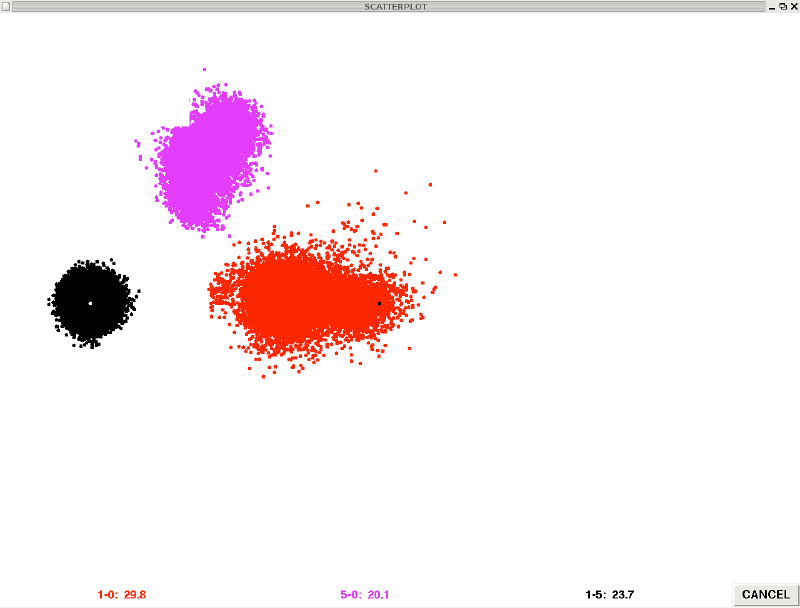
\includegraphics[width=\textwidth]{userguide-img006.png}}
  \captionof{figure}{Scatterplot projection from a 64-dimension space
    to 2-dimensions. These 2 clusters are probably not the same unit.}
  \label{scatter}
\end{center}

Each of the clusters in the scatterplot is multi-dimensional. Only a
\textit{slice} or plane can be viewed at one time.  The three points
used to define the plane of the scatterplot are the centers, or
averages, of the displayed clusters. The average of the noise is a
white dot, whereas the averages of the clusters are black
dots. \textit{Once clusters are merged, a new average is not
  determined; therefore, if merged clusters have an average dot, it is
  inaccurate; some merged clusters will not have an average dot, as
  seen in the purple cluster above.}  The color-coordinated numbers on
the bottom of the screen represent the distance between its
corresponding cluster and the noise. The numbers in black indicate the
distance between the clusters. In this example, Cluster 1, in red, is
29.8 units from the noise, while Cluster 5, in purple, is 20.1 units
from the noise. Clusters 1 and 5 are 23.7 units apart. \textbf{Note
  that spikes from the entire recording are displayed in the
  scatterplot, regardless of the Timeline display.}

\subsubsection{\sf DOUBLET details}
The {\sf DOUBLET} feature can be used if a cluster has an ISI less
than 2 ms. Such short ISIs may represent spikes from other
``contaminating'' neurons (under the assumption that one neuron cannot
have such a short ISI because of refractoriness). Alternatively, the
short ISIs may be represent one neuron firing with ``doublets'' or
short bursts of high frequency spiking. To help distinguish between
these alternatives, select a cluster and click the {\sf DOUBLET}
button. A raw data window will open displaying the first point in the
raw data where a spike fired within 2 ms of the previous spike. You
must determine if these spikes look similar and if the cell does
indeed appear to generate spikes with such a doublet or burst
pattern. When this button is pressed in succession, the window is
cleared and the next two spikes with an ISI less than 2 ms are
displayed. The number in the upper-left hand corner is roughly the
time at which the spikes occurred. Watch this when pressing the {\sf
  DOUBLET} button in succession to verify that you are not seeing the
same spikes again. The ``$\uparrow$'' key zooms out, allowing the user
to better compare the shape of the spikes. The ``$\downarrow$'' zooms
in and the ``$\leftarrow$'' and ``$\rightarrow$'' keys move the view
to earlier and later in the recording. To increase or decrease the
amplitude in the waveforms, use the ``+'' or ``$-${}'' keys on the
\textit{keyboard}.

\subsubsection{\sf MOVIE details}
\label{moviedetails}
The {\sf MOVIE} feature is quite useful to see how successive spikes
in a cluster are shaped and if they are (more or less) superimposed
upon one another. (Note: the {\sf MOVIE} feature displays \textit{raw}
spikes for selected channel(s) against the average waveform, so these
waveforms are different from the cluster waveforms displayed in the
Spike Sorter window, as described previously.) Because the traces are
displayed in succession, you are not seeing the activity in real
time. Any period of inactivity is not represented. The {\sf MOVIE}
function is also a useful tool for comparing the shapes of different
waveforms. The movie of one waveform is displayed in
\textbf{Fig. \ref{movie}}.  Use the ``+'' or ``$-${}'' keys (on the
\textit{keyboard}) to increase or decrease the amplitude in the
waveforms.
\begin{center}
  \makebox[\textwidth][c]{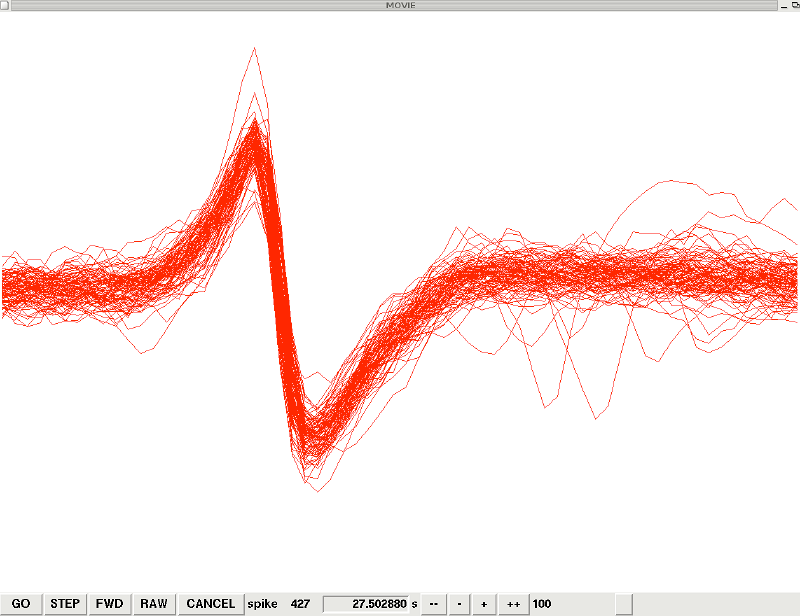
\includegraphics[width=\textwidth]{userguide-img007.png}}
  \captionof{figure}{Example of overlapping wave forms in a movie.}
  \label{movie}
\end{center}

The bottom of the Movie window includes the following function buttons:
\begin{description}
\item \textbf{\textsf {Go}} - starts the successive display of spikes
\item \textbf{\textsf {Step}} - changes the display one spike at a
  time
\item \textbf{\textsf {Fwd}} / \textbf{\textsf{Rev}} - spikes are
  displayed in forward or reverse chronological order
\item \textbf{\textsf {Raw}} / \textbf{\textsf{White}} - spikes are
  displayed in raw format or with a whitening process applied. The
  Spike Sorter looks at the waveforms in ``white'' format to assign
  spikes to clusters.
\item \textbf{\textsf {Cancel}} - closes the window
\item \textbf{\textsf {Spike \#}} - which spike is being displayed; \#
  of the spike in the edt file
\item \textbf{\textsf {\# s}} - time that this spike occurred within
  the recording
\item ``\textbf{\textsf {-- --}''} - displays the 64-sample segment of
  data immediately prior to the current data segment. Removes all
  other traces and leaves the average cluster waveform.
\item ``\textbf{\textsf {+ +}''} - displays the 64-sample segment of
  data immediately following the current data segment. Removes all
  other traces and leaves the average cluster waveform.
\item ``\textbf{\textsf {--}''} - moves the most recent trace to the
  right by one sample. Removes all other traces and leaves the average
  cluster waveform.
\item ``\textbf{\textsf {+}''} - moves the most recent trace to the
  left by one sample. Removes all other traces and leaves the average
  cluster waveform.

  (Note: The -- and + buttons actually move the 64-sample VIEWING
  WINDOW to the left and right one sample, respectively -- which moves
  the FEATURE or waveform position further along in the window or
  closer to the ``start'' of the 64-sample window.)
\item{\textbf{Number of waveforms being displayed at a time}} The
  \textit{default number} of waveforms displayed at a time is 100,
  \textit{in addition to} the average waveform.  This number can be
  changed by using the following keys:
  \begin{center}
    \begin{tabular}{cc}
      \centering{ $\leftarrow $} & { 1 waveform will be displayed at a time}\\
      \centering{ $\rightarrow $} & { 1,000 waveforms will be displayed at a time}\\
      \centering{ $\uparrow $} & { Increases the number displayed by one}\\
      \centering{ $\downarrow $} & { Decreases the number displayed by one}\\
      \centering{ {\sf Home}} & { Returns the number displayed to 100}\\
    \end{tabular}
  \end{center}
\end{description}

\subsubsection{Manually aligning waveforms}
\label{alignment}
The cluster waveforms in the Results panel (see section
\ref{overview}) each have a vertical dashed line showing the point in
time on the waveforms that will correspond to the spike times in the
{\tt .edt} file.  If the line is not marking the correct point on the
waveforms, you can move the waveforms by selecting the cluster (or
clusters) you want to move and using the left and right arrow keys to
move the waveforms until the line is marking the correct point.
\emph{Be careful that only the cluster(s) you want to move are
  selected.  Look at the list of selected cluster numbers on the
  Results panel before you move anything.}

Before merging clusters, each cluster must be properly aligned to its
own vertical dashed line so that the clusters will be properly aligned
to each other when they are merged.  Make sure all clusters are
properly aligned before clicking {\sf EDT} to write the final {\tt
  .edt} file.

The arrow keys move the waveforms one pixel at a time, so you can
position most precisely by expanding the window to full screen and
displaying just one cluster.  The arrow keys repeat, so you can hold
them down to move continuously.  A small window and lots of clusters
displayed will move fastest.

In addition to the waveform display and the {\tt .edt} file, shifting
the waveforms affects the movie, and less noticeably, the timeline,
ACH, and doublet functions.  The scatterplot is not affected.

The {\tt align} utility (Sec. \ref{align}) can be used to check that
proper spike time alignments got written to the {\tt .edt} file.

\subsubsection{Timeline}
\label{timeline}
The {\sf TLINE} function button displays firing rate histograms for
the recording (\textbf{Fig. \ref{tline}}), but only for the channels
that are displayed in the USF Spike Sorter window.
\begin{center}
  \makebox[\textwidth][c]{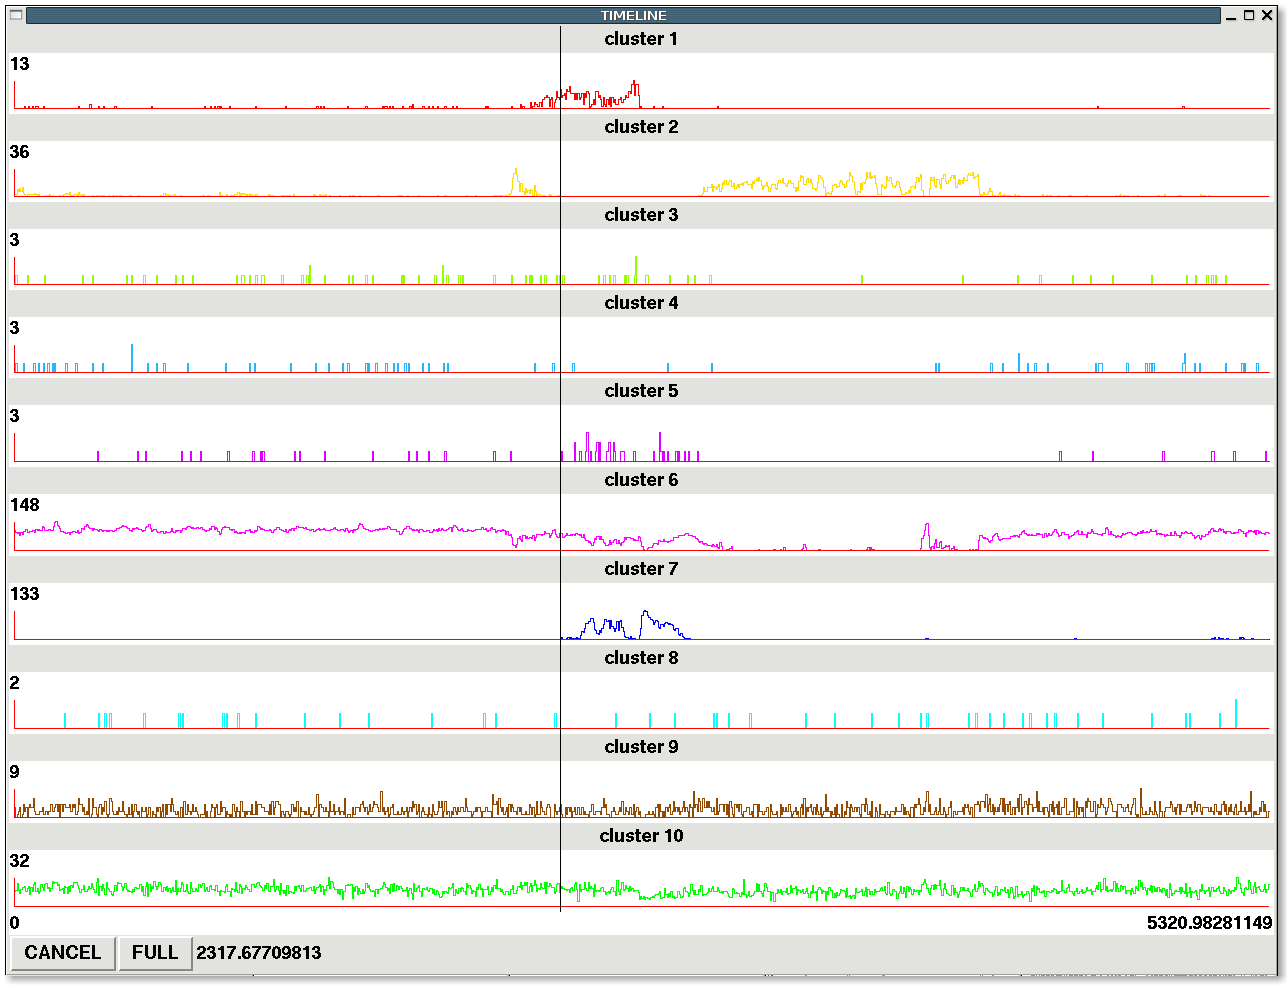
\includegraphics[width=\textwidth]{userguide-img008.png}}
  \captionof{figure}{Example of timeline display for clusters from a
    single electrode channel.}
  \label{tline}
\end{center}
The numbers on the left-hand side of each histogram represent the
number of spikes included in the highest peak of the histogram for
that cluster of waveforms. To select a particular part of the
recording and zoom in, move the mouse and click the beginning and the
end of the desired portion. To zoom out, left-click on the screen,
move the mouse to the right, then right-click. The display will be
compressed into the area between the left- and right-click lines, and
a longer period of time will be displayed. To see the entire
recording, click {\sf FULL}. \textbf{\textit{Note that the ACH, the
    raw display, and the movie will show data from the block of time
    displayed in the timeline.}} In some circumstances, the timeline
will not update after a change. To avoid this, click {\sf CANCEL} when
finished viewing.

\subsubsection{Example of results with timeline and scatterplot}
Another example using the tools is shown in \textbf{Fig. \ref{tools}.}
See captions associated with the figure.
\begin{center}
  \makebox[\textwidth][c]{\includegraphics[width=6in]{tools.jpg}}
  \captionof{figure}{One must pay careful attention to how spikes from
    one neuron are distributed in the clusters. Some of the spikes may
    be assigned to different clusters due to changes in shape even
    though we know the spikes are from the same cell. This may
    commonly occur over the course of a recording, with a single
    burst, or during an experimental perturbation.}
  \label{tools}
\end{center}

\subsection{Final thoughts on Evaluating-Manual sorting}
The process of Evaluating is complex, subjective and requires one to
understand that no two people will evaluate a channel exactly the same
way. The raw data, diagram, ACH, timeline, waveform, C/M/D assessment,
number of spikes, and scatterplot are all CLUES to whether a cluster
should be deleted, kept, or merged with another. It is suggested that
the {\sf NOTES} feature in the control panel is utilized to
communicate any important findings or issues and that screenshots be
made to refine or clarify your notes.

\subsection{Tips}

{\bfseries\itshape OK. Time to actually DO it ...}

Now that you've read about what each button will do, here are some
tips (and accompanying philosophies and gotchas) for manual spike
sorting, courtesy of Dr. Sarah Nuding. You will fall into your own
sorting rhythm as you become more familiar with the tools and
auxiliary programs, but the steps outlined here are a good place to
start.

\textbf{\textit{Things to keep in mind while sorting:}}

\begin{itemize}
\item First, open the {\sf RESULTS} panel and look at the initial
  clustering. The clusters you see when you first open the Results
  panel are NOT necessarily individual units! Indeed, \textbf{it is
    likely that several clusters and their associated waveforms
    constitute the spikes from a single neuron.} Sometimes two
  separate waveforms (units) are included within an original cluster.
\item Sometimes clusters will look as though 2 waveforms of
  approximately equal amplitude were caught together within the
  64-sample window; they may look like an ``M'' or a ``W''. This means
  that the 2 events were counted as 1 event -- and you're missing one
  of the events. Superimposed events like these will require further
  editing (e.g., {\tt dup\_ids}; see Section \ref{dup}) if you want to
  isolate both waveforms. If, however, one of the waveforms is much
  smaller than the other and you wouldn't be able to isolate it
  anyway, you can ignore the ``wart'' and isolate the larger
  waveform. The superimposition of a small unit over a bigger unit
  looks like a non-stationary ``wart'' (or ``fly'') moving over the
  larger unit's waveform over time. You can usually see this by
  viewing a movie of the data.
\item Second, evaluate the raw channel data to get an idea of how many
  units may be sortable. Remember that some of our recordings are very
  long. Sometimes there's a clear single unit, and yet the autosorting
  process may have put the waveforms for that unit into 50 separate
  clusters! And it may be that there aren't any real units, just
  noise. It's good to have an idea of what to expect before going in.
\begin{itemize}
\renewcommand{\labelitemii}{\ding{226}}
\item ``As for the Spike Sorter seeing lots of different clusters when
  we know it's really one{}---this happens mostly on the ``cleanest''
  channels{}---or the HUGE unit on the channel ending up in the last
  cluster and not sorted at all: As evaluators (and supposedly after
  looking through the raw data FIRST so you know this right away) this
  is ONE problem I love to have{}---sorting is SO easy on channels
  like that! If a person doesn't catch this, they really aren't ready
  to be left on their own.''
\end{itemize}

\item Delete the obvious, such as clusters that are in or touching
    the noise (look at the scatterplot) or waveforms that look like
    exponential decay. Aside from these, \textbf{don't delete any
      cluster until you are totally done with manual sorting.}
\begin{itemize}
\item The previous point bears repeating: Don't delete individual
  clusters just because they are labeled ``dirty'' or have a ``beach''
  in the ACH. Put all the clusters together that belong together (use
  movies, scatterplots, etc.). The decision to keep or discard the
  final, conglomerate cluster should be made at the end of the manual
  sorting process for this channel.
\item Let's put it this way: Say that clusters 1-5 belong together
  (you've looked at the raw data) and that all of those clusters are
  individually ``clean.'' Merging cluster 5 (which has, say, 5,000
  events) with cluster 1 (1,000 events) may result in a fair number of
  ISIs ${\leq}$ 2ms (perhaps 50 of the \~6,000 ISIs) or a
  wrong-looking ACH, so you think, ``I can't merge these 2 clusters
  together. Hmmm {\dots} maybe I should delete one of them.'' However,
  if you merge clusters 1, 2 (50,000 events), 3 (25,000 events) and 4
  (4,000 events) together first and \textit{then} merge in cluster 5,
  the resulting cluster will have at least the same number of ISIs
  ${\leq}$ 2ms, but now that's \~50 of 84,000 ISIs (not as bad,
  proportionately speaking) and the ACH may look much better, too --
  and now you may decide to keep the final merged cluster. {\tt
    autoCCH} will help with this decision ...
\end{itemize}
\item Use \texttt{autoCCH} (an auxiliary program run from the command
  line) to look at the original {\tt .edt} file produced during the
  Autosort process. (It may be useful to save the original {\tt .edt}
  file by changing its filename.) If two clusters whose spikes are
  intermingled with one another truly DO belong together, you will see
  a telltale gap at the origin even at large bin widths due to the
  refractory period in the cross-correlograms calculated from those 2
  spike trains. (This is not to be confused with the bin-thin artifact
  that usually occurs just because units were recorded on the same
  electrode.) This process may give you a good idea of which clusters
  should be merged -- and which ones definitely don't belong
  together. You may also create intermediate {\tt .edt} files to help
  along the way.
\item If they can't be separated into 2 separate clusters, then you
  can't keep the cluster or all the other clusters that belong with
  it. Remember, though -- don't make the decision to keep or delete
  until after you have merged all clusters that belong together.
\item Look at the autocorrelogram (ACH) for each cluster to identify
  clusters with many inter-spike intervals (ISIs) ${\leq}$ 2 ms in the
  ACH. A typical bin-width to make this determination is around 0.50
  ms (selected with the slider).  Typically, noise will have a huge
  number of counts early in the ACH. Noise usually has what looks like
  a monotonic descending (to the right) first-order autocorrelation
  histogram. Occasionally, there will be a small number of ISIs
  ${\leq}$ 2ms, but the likelihood that you have a ``good'' cluster is
  higher than the data assessment would indicate.  Remember -- merge
  the clusters that belong together before deciding to keep or delete
  a merged cluster.
\item You will assess ACHs throughout the sorting process as you
  decide whether to merge clusters. When assessing the shape of the
  ACHs at different bin-widths (resolutions), ``plateaus'' or regions
  that look like a beach near the histogram origin are indicators that
  the cluster includes spikes from more than one neuron (because
  refractoriness, except in the case of ``doublets'' and the like,
  precludes very short ISIs less than 2 ms). ACHs with low ISIs are an
  indicator to use other tools like the \textsf{MOVIE} to look at one
  or more clusters over a time interval of interest to see if more
  than one waveform is included in the cluster. At this point, you can
  switch back and forth between \textit{scatterplots} and
  \textit{movies} to look at the shape of the cluster over time. When
  viewing movies, select more than one cluster to see how similar they
  are or what their approximate ratio of occurrence is---very often a
  cluster will appear very rarely in relation to another selected
  cluster---and this facilitates the decision whether or not to merge
  the clusters.
\item Look at the \textsf{DIAGRAM} (generated from the \textsf{Control
    Panel}) and see which clusters are closer to each other (lower
  number on the arrow connecting them). The diagram represents the
  clusters as circles with arrows connecting them. Each arrow has a
  number associated with it and these numbers are ``distances''
  between the clusters in 64-space. Open the \textsf{RESULTS} panel to
  look at the clusters and see if you can merge them based on their
  shape, distance to the compared cluster, and ACH. Sometimes the
  diagram makes it easy to merge clusters more quickly.
\item Look at the \textsf{TIMELINE} for the entire data file and check
  the day sheets and chart records to determine which treatments were
  given to the animal (look for anomalies). If there is a
  physiological event or stimulus perturbation (like hypoxia), select
  a segment of the timeline that is relatively clean (like the
  ``control'' period) and exclude the treatment event. (Note: Anything
  NOT selected in the timeline will NOT be reflected in the ACHs.) Now
  go back to the main \textsf{RESULTS} screen to look at the resulting
  ACHs. At this point, you can make a more informed decision about
  which clusters are similar enough to merge and which are truly
  separate units/clusters.
\item You can zoom in on the \textsf{TIMELINE} and bring up the
  \textsf{RAW DATA} associated with that region of the timeline and
  stack the windows vertically to compare cluster spikes with raw
  data. This recommended approach shows the original spikes in
  relation to their counts in the histogram. Seeing the timing of any
  given spike both in the raw data and in the waveform timeline can
  aid in the decision process. (Note: If you do this, remember to
  reset your \textsf{TIMELINE} before you go back to the
  \textsf{RESULTS} panel so your ACHs represent the appropriate data.)
\item The superimposition of a small unit over a bigger unit looks
  like a non-stationary ``wart'' (or ``fly'') moving over the larger
  unit's waveform over time. You can usually see this by viewing a
  movie of the data.
\item \textit{Complete one channel in its entirety before moving to
    the next channel or submitting it for review.} That includes using
  auxiliary programs like {\tt autoCCH}, {\tt tmover}, and {\tt
    timedisedt} if necessary to completely separate the unit waveforms
  of one (or more) unit(s) from the noise and other waveforms.
\item ``Sometimes the Manual Sorting/Evaluation step for a channel can
  take an hour, sometimes it takes 2 days. I'll cut as many units as I
  can with confidence. With our nearly 3 hour recordings, I see no
  problem with ending up with more than 6 clusters for a single unit,
  especially when I have to do some edits before they are merged. Most
  clusters seem to attract one-spike stragglers here and there (seen
  as singletons in the timeline on either side of the main periods of
  activity) that truly DO NOT belong (are not the same waveform). If I
  want to keep the cluster, I find those buggers and get rid of them
  (via scope or a text editor) and before writing the final edt for
  that channel. Some of the channels can have 26 or more clusters in
  an \textit{interim} {\tt .edt} because I have to adjust the spike
  times to align the waveforms (misaligned waveforms can be detected
  in the Movie). The \textit{final} {\tt .edt} for a channel cannot
  have more than 26 clusters!''
\item ``I use a mix of raw traces/overlapping waveforms in movies,
  overlapping or nearly-overlapping activity on the timeline, and
  audio cues as well as having another terminal window open to look at
  CCHs (using the {\tt autoCCH} program) from ``intermediate'' {\tt
    .edt} files: Nothing tells you more quickly that 2 clusters with
  intermingled spike times don't belong together than when you look at
  them with {\tt autoCCH} and you don't see the refractory period on
  either side of 0.''
\item ``I try to pay no attention to the number of spikes---and I even
  try to disregard all the stats (MWRs, CCRs, etc.)  until the very
  last step. Sometimes you DO chuck a unit with few spikes (maybe
  $<100$!) because it will be too much work to carry it through for
  further analysis when there are no good responses, not enough spikes
  for respiratory analysis, and too few spikes to determine meaningful
  crosses---i.e., crosses that can be shown to be SIGNIFICANT.''
\end{itemize}

\iffalse
\subsection{ Editing}

{\color{black}
If you have two waveforms that look alike and you subtract one from the other, the remaining waveforms should be about
the level of noise in order to delete it.tion to their counts in the histogram. Seeing the timing of any given spike
both in the raw data and in the waveform timeline can aid in the decision process. (Note: If you do this, remember to
reset your \textit{Timeline }before you go back to the \textit{Results }panel so your ACHs represent the appropriate
data.) Want to completely finish a channel before moving to the next one or submitting it for review. Final edt
filename must be of the form expname\_chan.edt (2004-01-18\_001\_05.edt for channel 5)}

{\color{black}
FINAL EDITS: Add info re removing ``outliers'' or stragglers using tmover (move to 99, eg), scope. Also stuff about
alignment with timedisedt. Want to completely finish a channel before moving to the next one or submitting it for
review. Final edt filename must be of the form expname\_chan.edt (2004-01-18\_001\_05.edt for channel 5)}
\fi

\bigskip

\subsection{Reviewing}

After a channel has been evaluated, it can be ``Reviewed''. Currently,
this is done by only the most experienced members of the lab
(primarily Dr. Sarah Nuding). This \textbf{QC} process of having all
channels assessed by at least two people helps to ensure that
high-quality data are being passed onto the next step in data
analysis.

\newpage
\subsection{Finishing up a channel}

When all clusters have been evaluated and reviewed on a channel, do
the following:

In the {\sf RESULTS} window:
\begin{enumerate}
\item Write an {\tt *.edt} file. Click {\sf EDT}. A small window in
  the upper-right appears displaying how the clusters will be named in
  the {\tt *.edt} file. Currently, we do not change the names. Click
  {\sf WRITE EDT}.
\item Capture the Results screen (make a screenshot of it). Move the
  slider bar to the appropriate bin width so that the true shape of
  the ACHs can be best seen.

  (Note: We have been saving screenshots of waveforms, clusters, etc
  in a subdirectory within the data directory; e.g., the subdirectory
  {\tt screenshots} in the data directory {\tt
    /datamax/2004-01-18/}. PNG is a good format choice.)
\item Click {\sf QUIT}. The {\sf RESULTS} window will close.
\end{enumerate}
In {\sf Spikesort Control Panel}:
\begin{enumerate}[resume]
\item Click {\sf UPDATE}.
\end{enumerate}
\subsection{Merging}
When Autosort Processing, Evaluating, and Reviewing have been
completed for all channels, a merge file can be made.  This is a large
{\tt .edt} file containing all of the information from all of the
channels. Before merging data, always make sure \textbf{all}
Processing and Reviewing has been completed, {\tt *.edt} files for
each channel have been written, and merged channel numbers
assigned. NOTE: Be sure to check that the spreadsheet (in {\tt .xls}
format) for the array coordinates has been completed, reviewed for
accuracy, and is in the appropriate folder \textit{before} pressing
this button; Spike Sorter creates an {\tt *.info} file (needed for
further analysis) and it will not be able to do so if the coordinate
spreadsheet is incomplete.

To merge the data for an experiment:

\begin{enumerate}
\item Verify that the final {\tt .edt} file has been written for each
  channel, including the analog channels.
\item Verify that merged channels ranges have been assigned to the
  appropriate brainstem region (i.e., the {\tt *.num} file).
\item Verify that the coordinate spreadsheet has been created and
  QC'd. Please note that even though there is a spreadsheet (in the
  directory under {\tt /raid/experiments/} for that experiment), or
  even that it is named ``final,'' does \emph{not} necessarily mean
  that it has been QC'd.
\item Click {\sf MERGE}.
\end{enumerate}

\textbf{Note:} The maximum number of distinct spike trains that you
are allowed to derive from 1 channel is 26. If there is movement of
the brain, or substantial evoked or recruited activity, a number of
different neurons may be monitored sequentially over the course of the
recording. You are not likely to identify sets of clusters from more
than a few (1 to 3 or 4) distinct neurons for any interval in a
recording. And if you do, be very careful and skeptical, because
overlaps would likely be excessive, resulting in missed events --
distorting the results.

\clearpage
\section{Auxiliary Programs}
\label{aux}

\subsection{\tt tmover}

The tmover program takes a spike file as input and generates a spike
file as output, with one of the spike IDs changed during the specified
interval. Running it with no arguments gives this message:
\begin{verbatim}
usage: tmover oldid newid start_sec end_sec < in.edt > out.edt
\end{verbatim}
The spike file can be {\tt .edt} or {\tt .bdt}, and the output file
will be the same format as the input file. During the specified
interval from {\tt start\_sec} to {\tt end\_sec}, {\tt oldid} is
changed to {\tt newid}. Everything else remains the same. Spikes of
{\tt oldid} at times that coincide with {\tt start\_sec} or {\tt
  end\_sec} get changed to newid.

\subsection{\tt timedisedt}

The {\tt timedisedt} program offsets the event times in a {\tt .edt}
file. It prompts for the input {\tt .edt} file name and an integer
offset in .1 ms ticks, and writes the output to {\tt timedis.edt}. It
will fail if {\tt timedis.edt} already exists. The output is the same
as the input, except that the event times have had the specified
offset added to them, and if the resulting time is less than 0, the
event is dropped.

\subsection{\tt autoCCH}

{\tt autoCCH} is intended for use as a survey of data contained within
an {\tt .adt}, {\tt .bdt}, or {\tt .edt} file. It will compute
cross-correlation histograms of each pair of cells contained within
the file. Pairings are made ``automatically.'' The user may eliminate
cells from this automatic display, if desired. Data for each pair of
cells is displayed at four user-selected binwidths (default = 0.5,
1.5, 2.5, 5.5 msec.). Maximum number of signals = 120. Assigned ID
codes may range from 1 to 999.  The user may print the graphics window
or may save it in {\tt .ps} format for later importation into a
PC-based drawing program.

\subsection{\tt scope}

Scope is a spike train analysis utility program to visualize the times
of action potentials in simultaneously monitored neurons, other event
timing pulse codes, and associated analog signal. The program can
scan, edit, select and save sections of {\tt .edt} and {\tt .bdt}
files for subsequent analyses. Scope provides traditional
representations such as firing rate histograms and rectified and
filtered (``integrated'') records and has tools to add time marker
``codes'' and delete or select sections of the data for subsequent
analysis (e.g., results from a particular stimulus protocol). You can
use this to create files containing a subset of spike trains. For
example, you may need to remove a spike train from the {\tt .edt} file
for editing. In such a case, remember to not only save the individual
spike train but also the rest of the file with that channel
omitted. When the editing is completed, use the auxiliary program
\texttt{merge} (see Section \ref{merge}) to put the edited channel
back into the file.

\subsection{\tt crossings2pos}

{\tt crossings2pos} is a level (or threshold) detector. It can be
useful when you think the Spike Sorter is not catching large spikes
that you think belong together in one cluster. {\tt crossings2pos}
generates a {\tt .pos} file with spike times for use with the Spike
Sorter, from a {\tt .chan} file, based on positive-going crossings of
a specified threshold. Running it with no arguments gives this usage
message:

\makebox[\textwidth][c]{\tt usage: crossings2pos xxx.pos yyy.chan threshold cluster... > new.pos}

The program is intended to be used with file \texttt{xxx.pos} that has
been generated by Spikesorter from \texttt{yyy.chan}, but for which
simple threshold crossings would have done a better
job. \texttt{threshold} is a number between $-32768$ and $32767$
chosen by the user, typically by reading it off the waveform display
(using the {\sf RAW DATA} button or {\tt waveform.tcl}) as the fifth
number displayed at the top, when the cursor is positioned at what
looks like an appropriate threshold level. \texttt{cluster...} is a
space-separated list of cluster numbers in {\tt xxx.pos} that will be
left out of {\tt new.pos}. The first number in the list will be
re-used in {\tt new.pos} as the cluster number for the
threshold-crossing spikes. If the old {\tt .pos} file is deleted or
renamed or moved, the new {\tt .pos} file can be given the name of the
old one, and then it can be viewed in the spikesorter. The waveform
overlay for the new cluster will be wrong, as will scatterplots that
include it, but everything else (including the Movie) should work. An
example session might look like this:
\begin{verbatim}
cd 2004-01-25_001
mv -i 2004-01-08_001_11.pos 2004-01-08_001_11-orig.pos
crossings2pos 2004-01-08_001_11-orig.pos \
2004-01-08_001_11.chan 28000 1 2 3 4 5 > 2004-01-08_001_11.pos
\end{verbatim}
NOTE: Dr. N. recommends that you use {\tt crossings2pos} in the
following manner. Usually, at least some of the large waveforms you
want to pick off with this threshold detector will be Autosorted into
one or more clusters. The waveforms in the cluster created by {\tt
  crossings2pos} will not be correctly aligned to the waveforms in the
Autosorted clusters -- they will not overlay in the Movie with the
waveforms in the Autosorted cluster(s) and you will have to ``jigger''
their times to make them align. You will need those Autosorted
clusters so you can figure out how much to jigger, so run {\tt
  crossings2pos} in such a way that you will not replace them. Do this
by replacing a cluster that you know you will delete or have already
deleted (like one that's in the noise; let's pick cluster 27 as an
example). Now you can use {\tt autoCCH} (make a new {\tt .edt} file
first!)  to see how far apart the spike times are and use timedisedt
only on the replacement cluster you made with {\tt crossings2pos} to
bring it into alignment with the original Autosorted clusters. So, the
command line would look like this:

\makebox[\textwidth][c]{\tt crossings2pos 2004-01-08\_001\_11-orig.pos
  2004-01-08\_001\_11.chan 28000 27 > 2004-01-08\_001\_11.pos}

So now, the next time you open that channel in the {\sf RESULTS}
panel, the waveform overlay for the new cluster (which will be cluster
27 in this example) will be wrong (it will still show you the old
stuff that was in cluster 27), as will scatterplots that include it,
but everything else (including the Movie and the ACH) will reflect the
new cluster 27.  Run the Movie and be sure that the waveforms overlay
and that you haven't ``caught'' anything you want to throw back.  If
you're not satisified, run {\tt crossings2pos} with a different
threshold. Because you have saved the original {\tt .pos} file, and
you can run {\tt crossings2pos} several times with different
thresholds if necessary.

\subsection{\tt merge}
\label{merge}
Use merge to place an edited cluster or channel within an existing
{\tt .edt} file. Running it with no arguments gives this usage
message:
\begin{verbatim}
usage: merge input1.[eb]dt input2.[ed]dt > newfile.[ed]dt
\end{verbatim}
For example:

\makebox[\textwidth][c]{\tt merge 2004-01-08\_001\_11-no27.edt
  2004-01-08\_001\_11-edited27.edt > 2004-01-08\_001\_11-v2.edt}

\subsection{\tt waveform.tcl}
\label{wave}
\begin{verbatim}
usage: waveform.tcl CHANFILE [START [END]]
\end{verbatim}
Displays the raw data in {\tt CHANFILE} from {\tt START} to {\tt END}.
{\tt START} and {\tt END} are integer sample numbers.

The raw data display can be very helpful (visually as well as aurally)
in evaluating a channel.  To listen to the trace -- as in a live
experiment with an audio monitor -- press ``p''. To stop the audio,
press ``s''.  The numbers in the upper-left and -right corners are the
time of the recording in seconds at the beginning and end of the data
displayed. The number in the upper-middle is the numbers of seconds
being displayed. Use the up and down arrow keys to zoom in and out,
and the left and right arrows to scroll through the raw data.

\subsection{\tt dup\_ids}
\label{dup}
\begin{verbatim}
usage: dup_ids map_file edt_file > out_edt_file
\end{verbatim}
Changes each id specified in {\tt map\_file} that it finds in {\tt
  edt\_file} to the two id's specified in the first line of {\tt
  map\_file}, with the offsets specified for that id.  The first line
should contain two id's with a space between.  Each of the other lines
should contain an id, and two offsets in ticks separated by spaces.
The result is written to {\tt out\_edt\_file}.

\subsection{\tt align}
\label{align}
\begin{verbatim}
usage: align CHANFILE SPIKEFILE TRIGGER
\end{verbatim}
Displays a waveform overlay of the spike waveforms from {\tt CHANFILE}
corresponding to the spiketimes in {\tt SPIKEFILE} for the unit
specified by {\tt TRIGGER}.  A vertical red line marks the point on
the waveforms corresponding to the times in {\tt SPIKEFILE}.  A single
white waveform overlayed on the black spike waveforms is the mean of
the spike waveforms.  {\tt SPIKEFILE} should be an {\tt .edt} file.
({\tt align} should work with {\tt .bdt} files, but we are unlikely to
have a corresponding {\tt CHANFILE}.) Pressing ``q'' quits.

This may be useful for checking the alignment of spike times to
cluster wavforms, and the alignment to each other of clusters that
were merged in the Spikesorter.

\clearpage
\nocite{letelier2000spike}
\nocite{harris2000accuracy}

\bibliographystyle{apalike}
\bibliography{references}
\end{document}
